\documentclass[10pt,twocolumn]{article}

% ── Packages ─────────────────────────────────────────────────────────────────
\usepackage[utf8]{inputenc}
\usepackage[T1]{fontenc}
\usepackage[margin=2cm]{geometry}
\usepackage{graphicx}
\usepackage{booktabs}
\usepackage{multirow}
\usepackage{siunitx}
\usepackage{xcolor}
\usepackage{enumitem}
\usepackage{amsmath}
\usepackage{hyperref}
\usepackage{cleveref}
\usepackage{caption}
\usepackage{subcaption}

\sisetup{group-separator={,}, group-minimum-digits=4}

\hypersetup{
  colorlinks=true,
  linkcolor=blue!60!black,
  citecolor=blue!60!black,
  urlcolor=blue!60!black,
}

\captionsetup{font=small, labelfont=bf, skip=6pt}

% ── Title ────────────────────────────────────────────────────────────────────
\title{%
  Energy Efficiency of Locally-Hosted Open-Source LLMs\\
  on Automated Software Engineering Tasks%
}

\author{%
  % TODO: add authors and affiliations
  Anonymous Author(s)
}

\date{}

\begin{document}
\maketitle

% ═════════════════════════════════════════════════════════════════════════════
\begin{abstract}
Large language models (LLMs) are increasingly deployed as autonomous coding
agents, yet little is known about their energy footprint when running on local
GPU hardware. We benchmark three open-source LLMs of comparable
size---Mistral Small~24B, Gemma~3~27B, and Qwen~3.6~27B---on the
SWE-bench Lite dataset using the OpenHands agent framework, measuring
per-second GPU power draw on a single NVIDIA A100~80\,GB PCIe accelerator.
Qwen~3.6~27B resolves 51 of 87~evaluated instances (58.6\%), compared to
10/65 (15.4\%) for Mistral and 8/97 (8.2\%) for Gemma. Despite consuming
\num{12150}\,Wh of total GPU energy---roughly three times more than
Mistral---Qwen achieves the lowest energy cost per resolved instance
(238\,Wh vs.\ 421\,Wh). We find that all bugs resolved by Mistral are a
strict subset of those resolved by Qwen, and that 39 bugs are resolved
exclusively by Qwen. Analysis of tool-call patterns reveals distinct
problem-solving strategies: Mistral favors file editing (68\% of tool
calls), while Qwen relies predominantly on terminal commands (55\%).
Our results demonstrate that raw energy consumption is a misleading proxy
for efficiency, and that task-effectiveness-normalized metrics are necessary
for meaningful comparisons.
% TODO: refine abstract once final results are confirmed
\end{abstract}


% ═════════════════════════════════════════════════════════════════════════════
\section{Introduction}
\label{sec:intro}

The rapid adoption of LLM-based coding agents~\cite{%
% TODO: cite OpenHands, SWE-agent, Devin, etc.
} raises questions about their computational and environmental cost.
While API-hosted models amortize inference across data centers with
optimized batching and hardware utilization, an increasingly common
deployment mode is \emph{local hosting}: running open-weight models on
dedicated GPU hardware for reasons of data privacy, latency, or cost
control.

In this setting, the GPU is exclusively allocated to a single model,
and its power draw---typically \SIrange{200}{300}{\watt} for a
data-center accelerator---is borne entirely by the user.
Unlike API pricing, which abstracts energy into token costs, local
hosting exposes the physical energy budget directly.

We present an empirical study of three open-source LLMs, each in the
24--27\,B parameter range, running on identical hardware (a single
NVIDIA A100~80\,GB PCIe GPU) against the SWE-bench Lite
benchmark~\cite{%
% TODO: cite SWE-bench
}. Our contributions are:

\begin{enumerate}[leftmargin=*, nosep]
  \item A controlled comparison of task-completion effectiveness and
        GPU energy consumption across three models under identical
        conditions.
  \item Per-second GPU power telemetry (\num{153659}+ samples per run)
        enabling fine-grained energy attribution to individual task
        instances.
  \item Evidence that total energy consumption is a poor proxy for
        efficiency---the model consuming the most energy per run is
        also the most efficient per resolved bug.
  \item Analysis of agent behavioral differences (tool-usage patterns,
        iteration depth) and their correlation with both effectiveness
        and energy.
\end{enumerate}


% ═════════════════════════════════════════════════════════════════════════════
\section{Related Work}
\label{sec:related}

% TODO: expand with full citations

\paragraph{LLM-based coding agents.}
SWE-bench~\cite{%
% TODO
} introduced a benchmark of real-world GitHub issues for evaluating
autonomous coding agents. OpenHands~\cite{%
% TODO
} provides an open-source agent framework supporting multiple LLM
backends. Prior evaluations focus on resolve rates and token
efficiency; energy consumption has not been systematically measured.

\paragraph{Energy measurement of ML workloads.}
GPU energy measurement using NVML power queries has been validated as
accurate to within \SI{5}{\percent} of wall-outlet
measurements~\cite{%
% TODO
}. Prior work has quantified training energy~\cite{%
% TODO: cite Strubell et al., Patterson et al.
}, but inference energy for agentic workloads---where a single task
may involve dozens of LLM calls interspersed with tool
execution---remains under-explored.


% ═════════════════════════════════════════════════════════════════════════════
\section{Methodology}
\label{sec:method}

\subsection{Hardware and Software}
\label{sec:hardware}

All experiments run on a single Azure Standard\_NC24ads\_A100\_v4
virtual machine equipped with one NVIDIA A100~80\,GB PCIe GPU
(TDP \SI{300}{\watt}), 24~vCPUs, and \SI{220}{\giga\byte} RAM.
The software stack comprises vLLM~0.25.1 for model serving,
OpenHands SDK~v1.16.1
as the agent framework, and Docker containers for per-instance
sandboxed evaluation.

\subsection{Models}
\label{sec:models}

We evaluate three instruction-tuned models of comparable size,
summarized in \Cref{tab:models}:

\begin{table}[t]
  \centering
  \caption{Models under evaluation. All served via vLLM with
           \num{32768}-token context and no native tool calling.}
  \label{tab:models}
  \small
  \begin{tabular}{@{}lccc@{}}
    \toprule
    \textbf{Model} & \textbf{Params} & \textbf{dtype} &
      \textbf{tok/s (gen)} \\
    \midrule
    Mistral Small 24B & 24B & fp16 & 25.8 \\
    Gemma 3 27B       & 27B & bf16 & 17.9 \\
    Qwen 3.6 27B      & 27B & bf16 & 23.5 \\
    \bottomrule
  \end{tabular}
\end{table}

\subsection{Benchmark}
\label{sec:benchmark}

We use SWE-bench Lite, a curated subset of 300~instances from the
full SWE-bench dataset. Each instance is a real GitHub issue paired
with a test patch; the agent must produce a code patch that passes
the held-out tests. We attempt 100~instances per model
(\texttt{n\_limit=100}) with a maximum of 100~agent iterations per
instance.

\subsection{Energy Measurement}
\label{sec:energy}

GPU power is sampled at \SI{1}{\hertz} via \texttt{nvidia-smi}
throughout each run, yielding a continuous power trace.
Total energy for a phase~$p$ is computed as:
\begin{equation}
  E_p = \sum_{t \in p} P(t) \cdot \Delta t
  \label{eq:energy}
\end{equation}
where $P(t)$ is the instantaneous GPU power at time~$t$ and
$\Delta t = \SI{1}{\second}$.

An idle baseline measurement is taken before each run
(GPU loaded with model weights but no active inference).
Baseline power ranges from \SIrange{43}{45}{\watt} across runs.
Net energy is computed by subtracting the idle baseline.

Per-instance energy is derived from the power trace using each
instance's start and end timestamps:
\begin{equation}
  E_i = \bar{P}_i \cdot d_i / 3600
  \label{eq:instance_energy}
\end{equation}
where $\bar{P}_i$ is the mean GPU power during instance~$i$ and
$d_i$ is the duration in seconds.


% ═════════════════════════════════════════════════════════════════════════════
\section{Results}
\label{sec:results}

\subsection{Task Completion}
\label{sec:completion}

\Cref{tab:outcomes} summarizes the fate of 100~attempted instances
per model. \Cref{fig:outcomes} visualizes the outcome distribution.

\begin{table}[t]
  \centering
  \caption{Instance outcomes. Each model attempted 100
           SWE-bench Lite instances.}
  \label{tab:outcomes}
  \small
  \begin{tabular}{@{}lrrr@{}}
    \toprule
    & \textbf{Mistral} & \textbf{Gemma} & \textbf{Qwen} \\
    \midrule
    Attempted       & 100  & 100 & 100 \\
    Timed out       &  35  &   3 &  13 \\
    Empty patch     &   1  &  15 &   0 \\
    Evaluated       &  65  &  97 &  87 \\
    \textbf{Resolved} & \textbf{10 (15.4\%)} & \textbf{8 (8.2\%)}
                       & \textbf{51 (58.6\%)} \\
    \bottomrule
  \end{tabular}
\end{table}

\begin{figure}[t]
  \centering
  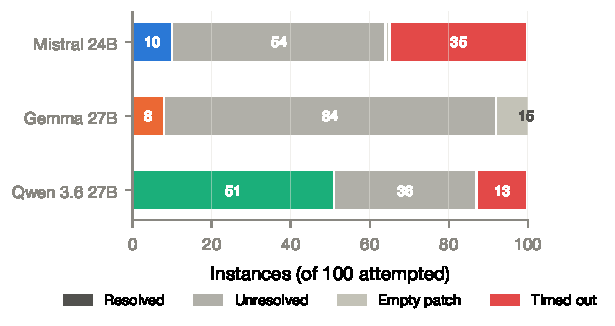
\includegraphics[width=\columnwidth]{figures/fig_outcomes.pdf}
  \caption{Instance outcome breakdown per model. The resolved segment
           (colored) uses each model's identifying color; gray shades
           indicate unresolved and empty-patch instances; red indicates
           timeouts. Mistral loses 35\% of instances to timeouts before
           producing any patch, while Gemma produces output for 97
           instances but 15 patches are empty.}
  \label{fig:outcomes}
\end{figure}

Qwen~3.6~27B substantially outperforms both other models, resolving
\num{51} of \num{87}~evaluated instances (58.6\%). Mistral resolves
\num{10}/\num{65} (15.4\%) and Gemma \num{8}/\num{97} (8.2\%).

The models exhibit distinct failure modes. Mistral times out on 35 of
100~instances without producing any patch, suggesting it frequently
enters unproductive loops. Gemma rarely times out (3/100) but produces
15~empty patches, indicating it reaches the \texttt{finish} action
without making code changes. Qwen has 13~timeouts and zero empty
patches.

\subsection{Resolved Instance Overlap}
\label{sec:overlap}

\Cref{fig:venn} shows the overlap of resolved instances across
models. Notably:

\begin{itemize}[nosep, leftmargin=*]
  \item All \num{10} bugs resolved by Mistral are also resolved by
        Qwen---Mistral's resolved set is a strict subset.
  \item \num{39} bugs are resolved exclusively by Qwen.
  \item Only \num{5} bugs are resolved by all three models.
  \item \num{1} bug (\texttt{django-15061}) is resolved by Gemma but
        not by Qwen, suggesting complementary strengths in rare cases.
\end{itemize}

\begin{figure}[t]
  \centering
  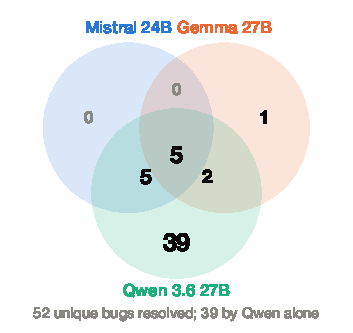
\includegraphics[width=0.92\columnwidth]{figures/fig_venn.pdf}
  \caption{Venn diagram of resolved instances. Qwen resolves a strict
           superset of Mistral's solutions and 39~bugs that no other
           model can fix. The union across all models is 52~unique
           bugs.}
  \label{fig:venn}
\end{figure}

\subsection{Energy Consumption}
\label{sec:energy_results}

\Cref{tab:energy} presents the energy measurements and
\Cref{fig:energy} visualizes the comparison.

\begin{table}[t]
  \centering
  \caption{Energy consumption and efficiency metrics.}
  \label{tab:energy}
  \small
  \begin{tabular}{@{}lrrr@{}}
    \toprule
    & \textbf{Mistral} & \textbf{Gemma} & \textbf{Qwen} \\
    \midrule
    Total runtime (h)       & 16.5  &  8.3  & 42.7  \\
    Avg GPU power (W)       & 255   & 198   & 285   \\
    Total GPU energy (Wh)   & \num{4211} & \num{1654} & \num{12150} \\
    Net energy (Wh)         & \num{3500} & \num{1295} & \num{10247} \\
    \midrule
    Energy / resolved (Wh)  & 421   & 207   & 238   \\
    Net energy / resolved   & 350   & 162   & 201   \\
    \bottomrule
  \end{tabular}
\end{table}

\begin{figure}[t]
  \centering
  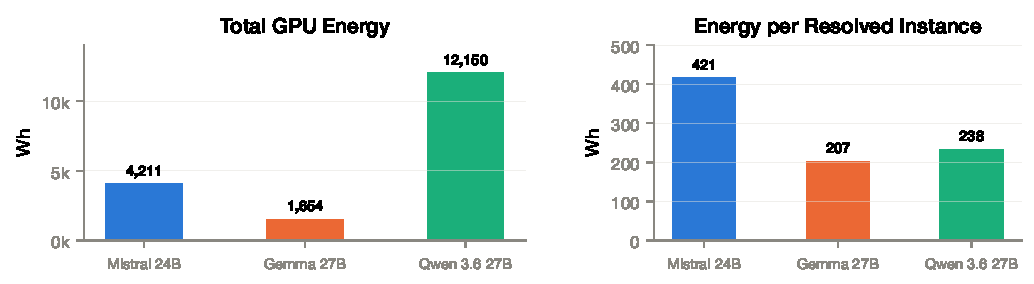
\includegraphics[width=\columnwidth]{figures/fig_energy.pdf}
  \caption{Left: total GPU energy per run. Right: energy per resolved
           instance. Despite consuming $\sim$3$\times$ more total
           energy, Qwen achieves a lower cost per resolved bug than
           Mistral (238 vs.\ 421\,Wh), because it resolves
           $\sim$5$\times$ more instances.}
  \label{fig:energy}
\end{figure}

Qwen consumes \num{12150}\,Wh of GPU energy over 42.7~hours---nearly
three times Mistral's \num{4211}\,Wh and seven times Gemma's
\num{1654}\,Wh. However, when normalized by the number of resolved
instances, Qwen is \emph{more} efficient than Mistral
(238 vs.\ 421\,Wh per resolved instance) because its 5$\times$~higher
resolve rate more than compensates for its higher absolute consumption.

Gemma achieves the lowest energy per resolved instance (207\,Wh) due
to its short average instance duration (\SI{159}{\second}) and low
average GPU power (\SI{198}{\watt}). However, its low resolve rate
(8.2\%) means the vast majority of energy is spent on unsuccessful
attempts.

\subsection{Instance-Level Analysis}
\label{sec:instance}

\Cref{fig:duration} shows the distribution of per-instance durations,
split by outcome. Across all three models, resolved instances complete
faster than unresolved ones:

\begin{itemize}[nosep, leftmargin=*]
  \item \textbf{Mistral:} median \SI{60}{\second} (resolved) vs.\
        \SI{102}{\second} (unresolved).
  \item \textbf{Gemma:} median \SI{42}{\second} vs.\
        \SI{111}{\second}.
  \item \textbf{Qwen:} median \SI{219}{\second} vs.\
        \SI{425}{\second}.
\end{itemize}

This pattern suggests that models ``know when they're stuck''---failed
instances consume more iterations and time before the agent reaches
the iteration limit or produces an incorrect patch.

\begin{figure*}[t]
  \centering
  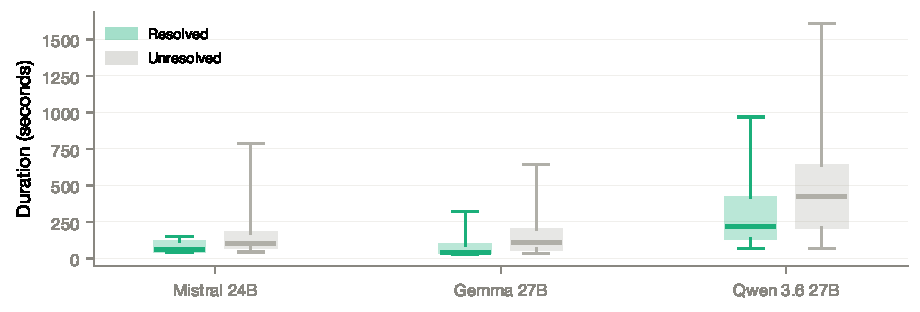
\includegraphics[width=\textwidth]{figures/fig_duration.pdf}
  \caption{Per-instance duration distributions, split by resolved
           (green) and unresolved (gray). Resolved instances are
           consistently faster across all models. Qwen's higher
           absolute durations reflect deeper exploration per instance
           (more tool calls, longer conversations), not idle time.}
  \label{fig:duration}
\end{figure*}

Qwen's durations are markedly longer than the other two models
(median \SI{219}{\second} vs.\ $\sim$\SI{60}{\second}).
This reflects deeper per-instance exploration: Qwen averages
16.4~tool calls over 18.6~turns per instance, compared to Mistral's
23.9~tool calls over 18.9~turns. Despite fewer tool calls, Qwen
spends more time because each interaction involves longer
conversations and more computation-heavy terminal commands.

\subsection{Tool Usage Patterns}
\label{sec:tools}

\Cref{fig:tools} shows the distribution of tool calls across models.

\begin{figure}[t]
  \centering
  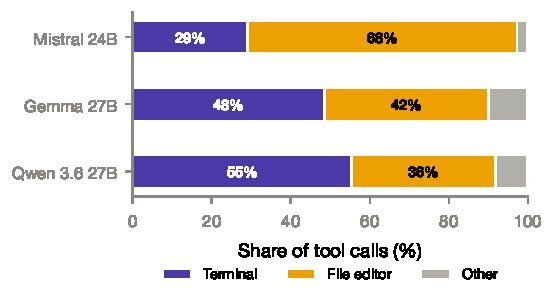
\includegraphics[width=\columnwidth]{figures/fig_tools.pdf}
  \caption{Tool-call distribution per model. Mistral is
           file-editor-dominant (68\%), while Qwen and Gemma favor
           terminal commands (55\% and 49\%, respectively). Higher
           terminal usage correlates with Qwen's deeper exploration
           and higher resolve rate.}
  \label{fig:tools}
\end{figure}

Mistral's tool usage is dominated by file editing (68\% of all calls),
with only 29\% terminal commands. This suggests a strategy of
directly modifying source files with less exploratory testing.
Qwen reverses this ratio (55\% terminal, 36\% file editor), indicating
a more test-driven workflow: running existing tests, exploring the
codebase with \texttt{grep} and \texttt{find}, and iteratively
validating changes.

\Cref{tab:full_comparison} provides a complete side-by-side summary
of all collected metrics.

\begin{table*}[t]
  \centering
  \caption{Full comparison of all benchmark metrics across the three
           models. All models ran on the same hardware
           (A100~80\,GB PCIe, TDP \SI{300}{\watt}) with identical
           agent configuration (\texttt{n\_limit=100},
           \texttt{max\_iterations=100}).}
  \label{tab:full_comparison}
  \small
  \begin{tabular}{@{}llrrr@{}}
    \toprule
    \textbf{Category} & \textbf{Metric}
      & \textbf{Mistral Small 24B} & \textbf{Gemma 3 27B}
      & \textbf{Qwen 3.6 27B} \\
    \midrule
    \multirow{5}{*}{Completion}
      & Attempted              & 100        & 100        & 100         \\
      & Timed out              &  35        &   3        &  13         \\
      & Empty patch            &   1        &  15        &   0         \\
      & Evaluated              &  65        &  97        &  87         \\
      & \textbf{Resolved}      & \textbf{10 (15.4\%)} & \textbf{8 (8.2\%)}
                               & \textbf{51 (58.6\%)}               \\
    \midrule
    \multirow{4}{*}{Performance}
      & Gen throughput (tok/s)    & 25.8     & 17.9     & 23.5       \\
      & Prompt throughput (tok/s) & 158.3    & 188.4    & 433.0      \\
      & KV cache utilization (\%) & 7.9      &  5.6     &  6.8       \\
      & Total tokens (M)          & 21.1     & 29.0     & 30.2       \\
    \midrule
    \multirow{4}{*}{Energy}
      & Total runtime (h)        & 16.5     &  8.3     & 42.7       \\
      & Avg GPU power (W)        & 255      & 198      & 285        \\
      & Total GPU energy (Wh)    & \num{4211} & \num{1654} & \num{12150} \\
      & Energy / resolved (Wh)   & 421      & 207      & 238        \\
    \midrule
    \multirow{3}{*}{Behavior}
      & Avg tool calls / inst.   & 23.9     & 15.8     & 16.4       \\
      & Terminal share (\%)      & 29.1     & 48.5     & 55.4       \\
      & File editor share (\%)   & 68.2     & 41.6     & 36.4       \\
    \midrule
    \multirow{4}{*}{\shortstack[l]{Instance\\duration (s)}}
      & Avg (all)                & 144      & 159      & 397        \\
      & Median resolved          &  60      &  42      & 219        \\
      & Median unresolved        & 102      & 111      & 425        \\
      & Max                      & 788      & 643      & \num{1610} \\
    \bottomrule
  \end{tabular}
\end{table*}


% ═════════════════════════════════════════════════════════════════════════════
\section{Discussion}
\label{sec:discussion}

\paragraph{Absolute vs.\ normalized energy.}
Our central finding is that total energy consumption is a misleading
measure of efficiency for agentic workloads.
Qwen consumes $\sim$3$\times$ Mistral's total energy but resolves
$\sim$5$\times$ more bugs, yielding a 44\% lower energy cost per
resolved instance.
This parallels findings in other domains where
effectiveness-normalized metrics (e.g., energy per correctly
classified image) invert na\"ive rankings based on total
consumption~\cite{%
% TODO
}.

\paragraph{The cost of failure.}
Unresolved instances are not free---they consume GPU energy without
producing value. Across all models, unresolved instances take longer
(higher median duration) and consume more energy than resolved ones.
Mistral's 35\% timeout rate represents substantial wasted energy:
these instances consumed power for the full iteration budget without
producing any patch. An early-exit heuristic that detects
unproductive loops could significantly reduce waste.

\paragraph{Strategy and effectiveness.}
The tool-usage analysis reveals that higher resolve rates correlate
with more terminal-heavy strategies. Qwen's preference for running
tests and exploring the codebase via terminal commands (55\% of tool
calls) suggests a more effective debugging workflow than Mistral's
file-editing-dominant approach (68\%). This aligns with software
engineering best practices where understanding the failure mode
through testing precedes fixing the code.

\paragraph{Model complementarity.}
Despite Qwen's dominance, Gemma resolves one instance
(\texttt{django-15061}) that Qwen does not, suggesting that model
ensembles or cascading strategies could further improve coverage.
The union of all three models' resolved sets is 52~bugs---only one
more than Qwen alone---indicating limited complementarity in this
size class.

\paragraph{Limitations.}
Our study has several limitations:
\begin{itemize}[nosep, leftmargin=*]
  \item We evaluate only three models in a narrow parameter range
        (24--27\,B). Smaller or larger models may show different
        energy--effectiveness trade-offs.
  \item SWE-bench Lite contains exclusively Python projects. Energy
        profiles may differ for other languages or task types.
  \item We measure GPU power only; CPU, memory, and network energy
        are excluded. GPU power dominates
        ($>\SI{80}{\percent}$ of system draw under load) but total
        system energy would be higher.
  \item Per-instance energy attribution uses averaged power over the
        instance duration, which may under- or overcount during
        periods of mixed GPU utilization (e.g., concurrent Docker
        operations).
  \item We run a single trial per model. Stochastic variation in
        LLM outputs means individual instance outcomes may differ
        across runs.
\end{itemize}


% ═════════════════════════════════════════════════════════════════════════════
\section{Conclusion}
\label{sec:conclusion}

We present the first controlled energy benchmark of locally-hosted
open-source LLMs on autonomous coding tasks.
Our results demonstrate that:
(1)~task effectiveness varies dramatically across models of similar
    size, with Qwen~3.6~27B resolving 51/87 instances (58.6\%)
    vs.\ $\leq$15.4\% for the other two models;
(2)~total energy consumption is a poor proxy for efficiency---the
    most energy-consuming model achieves the lowest cost per resolved
    bug;
(3)~distinct tool-usage strategies (terminal-heavy vs.\
    editor-heavy) correlate with effectiveness; and
(4)~resolved instances complete faster than unresolved ones,
    suggesting that early-exit mechanisms could reduce energy waste.

These findings argue for reporting energy-per-resolved-task alongside
raw resolve rates in future coding-agent benchmarks, and for
developing energy-aware agent strategies that can terminate
unproductive attempts early.

% TODO: add acknowledgments and data availability statement


% ═════════════════════════════════════════════════════════════════════════════
% \section*{Acknowledgments}
% TODO

% ═════════════════════════════════════════════════════════════════════════════
\bibliographystyle{plain}
% \bibliography{references}
% TODO: create references.bib and uncomment

\end{document}
